\documentclass[10pt,journal,compsoc]{IEEEtran}
\usepackage{amsmath,amssymb,amsthm}
\usepackage{booktabs}
\usepackage{graphicx}
\usepackage{xcolor}
\usepackage{algorithm}
\usepackage{algorithmic}
\PassOptionsToPackage{hyphens}{url}
\usepackage[hidelinks]{hyperref}

\newtheorem{definition}{Definition}
\newtheorem{theorem}{Theorem}
\newtheorem{proposition}{Proposition}
\newtheorem{corollary}{Corollary}

\begin{document}

\title{SEAL: Statistically-Bounded Erasure Audits for Machine Unlearning under Mutual Distrust}

\author{Quang-Vinh~Dang
\thanks{Q.-V. Dang is with British University Vietnam, Hung Yen, Vietnam (e-mail: vinh.dq4@buv.edu.vn). ORCID: 0000-0002-3877-8024.}
}

\markboth{IEEE Transactions on Information Forensics and Security}{}

\maketitle

\begin{abstract}
A data owner who submits an erasure request to a machine learning system operator has no direct way to verify that the request was honored, and the operator has no incentive to volunteer proof of noncompliance. Prior work shows that any audit accurate enough to catch a dishonest operator necessarily leaks information about the retained population, but stops short of a mechanism a mutually distrusting pair can actually run. This paper presents SEAL, a two-channel erasure-audit certificate that separates a zero-privacy-cost check on the data owner's own forgotten records from a differential-privacy-bounded check on synthetic boundary probes, calibrated against replicated honest re-executions rather than assumed thresholds, and its counterpart SEAL-W for large language model unlearning, which retrieves a randomly chosen member of a paraphrased query cluster through real Paillier-based private information retrieval and cross-checks response diversity against a phantom-topic baseline. We state five formal results (four theorems and a proposition) -- mostly standard tools (a two-hybrid IND-CPA reduction, a hypergeometric evasion bound, an exact Student-$t$ predictive threshold, Boole's inequality) applied to this certificate's specific channels, not new mathematics -- precisely scoping what each channel provably defeats: private information retrieval obliviousness under the decisional composite residuosity assumption, a hypergeometric bound on a resource-limited adversary's evasion probability, an exact finite-sample calibrated threshold, a zero-diversity guarantee against uniform response suppression, and a Bonferroni-corrected composition bound whose violation we found in our own implementation, and fixed, by writing this proof down. We reproduce the verification methodology of WaterDrum, the closest prior watermark-based unlearning audit, as an explicit baseline over 30 trials: a server that detects and filters the audit query itself defeats the WaterDrum-equivalent single-query check every time (0\% detection), the exact gap WaterDrum's own authors report as unsolved, while the full SEAL-W certificate catches it 93\% of the time once calibrated with a sufficient replicate budget -- a full sweep of that budget, not just this endpoint, is reported rather than only the flattering value. This 93\% figure is also the easiest case for our diversity channel, since uniform query suppression provably drives the true signal to exactly zero (Proposition~\ref{prop:zerodiv}); a harder, resource-bounded variant of the same attack that does not carry this guarantee is caught only 20\% of the time, against a 40\% analytic ceiling. Experiments on federated logistic regression over UCI German Credit, MNIST, and a 150{,}000-row Forest Covertype subsample, and on a real fine-tuned language model audited over the real TOFU fictitious-author benchmark, report both power and honestly-measured failure modes at small calibration-sample sizes, rather than tuning them away.
\end{abstract}

\begin{IEEEkeywords}
Machine unlearning, differential privacy, private information retrieval, text watermarking, auditing, federated learning, right to be forgotten.
\end{IEEEkeywords}

\section{Introduction}

Data-protection regulation gives individuals a right to have their data erased from systems trained on it \cite{gdpr2016}. When the system is a machine-learned model, ``erasure'' is a claim about a training procedure the data owner cannot observe: the model operator asserts that a retraining or fine-tuning step removed the record's influence, and the data owner must decide whether to believe it. This is not a benign estimation problem. The operator may find honest unlearning expensive and have every incentive to claim compliance while changing nothing (\emph{lazy} noncompliance), or to narrowly patch only the behavior an audit is expected to probe while leaving the record's broader influence untouched (\emph{targeted spoofing}).

Two recent results sharpen why this is hard rather than merely inconvenient. Tang, Joshi, and Kundu give an information-theoretic argument that, for convex models, any audit relying only on the model's behavior (query-response pairs) cannot separate an honestly-unlearned model from an insufficiently-unlearned one without revealing membership information about the retained set \cite{tang2026geometric} -- there is an unavoidable trade-off between how powerful a behavioral audit is and how much it leaks about records the data owner was never entitled to see. Nguyen et al.'s veriFUL framework independently surveys the federated-unlearning-verification landscape and concludes that no proposed scheme yet gives a federation of mutually distrusting clients and servers a concrete, run-once verification protocol with a stated privacy cost \cite{nguyen2025veriful}. Both papers characterize the problem; neither gives an auditor a mechanism to run.

\subsection{Contributions}

This paper's contribution is a concrete audit protocol -- not a new impossibility result, and not a claim to have invented differential privacy, private information retrieval (PIR), or text watermarking. It is the specific combination of known primitives into a certificate that (i) makes the audit power/privacy-leakage trade-off in \cite{tang2026geometric} a dial the data owner turns rather than an unavoidable fact they simply accept, and (ii) instantiates that dial concretely for two settings veriFUL leaves open: federated classical-ML unlearning, and large-language-model unlearning verified via watermarking. Concretely:

\begin{enumerate}
\item A two-channel certificate (SEAL) that separates a \emph{zero-marginal-privacy-cost} channel -- the data owner re-evaluates the model on data it already possesses in full, which costs no retained-set privacy at all -- from a \emph{tunable-privacy-cost} channel using Gaussian-mechanism-noised synthetic boundary probes, whose spend is set by a stated $(\varepsilon,\delta)$ budget (Section~\ref{sec:seal}).
\item A calibration procedure that builds each channel's null distribution from literal re-executions of the honest mechanism, matched to the real run's seed and per-client ordering, rather than an assumed parametric null -- a detail shown empirically not optional (Section~\ref{sec:seal}).
\item SEAL-W, a watermark-based certificate for LLM unlearning that plants several independently-paraphrased queries about the same forgotten entity in a committed batch, retrieves one at random via real Paillier-based PIR, and adds an independent response-diversity channel targeting exactly the adversary class -- uniform, topic-level output filtering -- that a single-query watermark check structurally cannot catch (Section~\ref{sec:sealw}).
\item Five formal results (four theorems and a proposition), precisely scoping -- not inventing -- what each channel is proven to defeat (Section~\ref{sec:theory}; full derivations in the supplemental material). Four combine standard tools (a two-hybrid IND-CPA reduction, the hypergeometric distribution, an exact Student-$t$ predictive interval via Cochran's theorem, Boole's inequality) with this certificate's specific channels, rather than proving new mathematics; their value is precision about scope, not proof difficulty. The fifth, the Bonferroni composition bound, found something we did not already know before proving it: a violation present in our own first implementation, caught by writing the proof down rather than by an experiment failing visibly, and fixed prior to the experiments reported here.
\item An explicit reproduction of WaterDrum's verification methodology \cite{lu2026waterdrum} as a first-class baseline over 30 trials, showing it is defeated every time by exactly the server behavior its own authors report as an open problem, against a 93\% detection rate for SEAL-W once its calibration budget is raised as this paper's own diagnosis prescribes -- reported alongside the smaller, inconclusive gap an earlier, under-calibrated configuration produced, so the improvement is shown, not only claimed (Section~\ref{sec:waterdrum-comparison}).
\item An empirical evaluation (Section~\ref{sec:experiments}) on three classical-ML datasets spanning three orders of magnitude in per-client data volume, and on a real fine-tuned language model audited over the real TOFU fictitious-author benchmark \cite{maini2024tofu}, reporting failure modes -- including a benchmark-scale finding that audit power \emph{degrades} as per-client data grows -- as honestly as the successes.
\end{enumerate}

Every individual primitive reused here -- zero-concentrated differential privacy (zCDP) accounting \cite{bun2016concentrated}, Paillier-based PIR \cite{paillier1999}, the Kirchenbauer et al. green-list watermark \cite{kirchenbauer2023watermark}, and RESPIR's oblivious-audit-via-PIR pattern \cite{godinot2026respir} -- is standard and cited rather than re-derived. What is new is their specific composition into a certificate answering a stated open problem in the unlearning-verification literature, and the formal accounting of exactly which adversary class each piece defeats.

\section{Related Work}
\label{sec:related}

\subsection{Unlearning Verification under Mutual Distrust}

Machine unlearning itself -- the underlying capability SEAL audits, rather than provides -- has an extensive literature independent of any audit mechanism, starting with Cao and Yang's original formulation of unlearning as a summation-form retraining problem \cite{cao2015towards}. SISA training \cite{bourtoule2021sisa} restructures training into isolated, retrainable shards, trading a constant-factor storage/computation overhead for an exact retraining guarantee; Guo et al.'s certified removal \cite{guo2020certified} and Sekhari et al.'s follow-up \cite{sekhari2021remember} instead give approximate, statistically certified guarantees for convex (or convex-adjacent) models via bounded parameter perturbation, avoiding retraining but only for the model classes their analysis covers. None of these three addresses verification: each assumes the deleting party is honest and asks only how to delete efficiently. The federated setting has the same gap -- Liu et al.'s FedEraser \cite{liu2021federaser} accelerates client-level retraining by reusing cached updates, again assuming an honest server -- and Gao et al.'s VeriFi \cite{gao2024verifi} and Sommer et al.'s Athena \cite{sommer2022athena} are the closest verification-side proposals: VeriFi unifies several federated-unlearning/verification-method combinations into one empirical framework, while Athena gives a client a backdoor-membership-inference test against a claimed-forgotten model. Both, like WaterDrum (below), assume a non-adaptive or honest-but-curious server rather than SEAL's actively adversarial threat model (Section~\ref{sec:threat}), and neither states a controllable privacy cost for the check itself -- Table~\ref{tab:relatedwork} records this gap alongside the comparisons that follow. Thudi et al.\ give an earlier, complementary caution: without a fixed, auditable definition of the training algorithm, \emph{any} behavioral observation of ``was this point unlearned'' is inherently ambiguous, since the same output distribution can arise from different training histories \cite{thudi2022necessity}. SEAL and SEAL-W sidestep this by construction: both compare post-request behavior against a calibration distribution built from literal re-executions of the \emph{same}, fixed honest mechanism, pinning the null hypothesis to one concrete algorithm rather than an unspecified space of behaviorally-equivalent ones.

Tang, Joshi, and Kundu's geometric transfer theorem \cite{tang2026geometric} is, to our knowledge, the sharpest existing formal statement of why this problem is hard: for convex models, it derives a per-point lower bound relating a behavioral audit's accuracy to the leakage it must incur on a named retained point, and shows this bound is essentially tight for the class of audits it covers. It is a \emph{characterization} result -- it says what any sufficiently powerful behavioral audit must cost, not how to build one that spends that cost deliberately, chooses where to spend it, or composes multiple audit channels with different leakage profiles. Nguyen et al.'s veriFUL survey \cite{nguyen2025veriful} independently reaches the same practical conclusion from the federated-learning side: after cataloguing verification entities, goals, and metrics proposed across the federated-unlearning literature, it concludes that none of the surveyed schemes gives a federation of mutually distrusting clients and servers a concrete, run-once protocol with a stated, controllable privacy cost. Neither paper is in tension with SEAL's design; SEAL is best read as an attempt at the mechanism both papers imply is missing, evaluated against the specific adversary classes (lazy noncompliance, targeted spoofing) that motivate their impossibility and survey arguments respectively. Sarmasarkar et al.'s contemporaneous auditor \cite{sarmasarkar2026auditing} takes a complementary approach: data-dependent lower bounds on an unlearning mechanism's effective $\varepsilon$ via membership inference, distinguishing rigorous removal from empirical methods that leave a detectable trace -- but with a single auditor holding model access, not SEAL's mutually-distrusting, query-only setting, and no bound on what the auditing itself leaks.

González et al.'s sequential auditing framework \cite{gonzalez2025sequential} solves an adjacent but structurally different problem: given repeated, i.i.d.\ access to a mechanism under two auditor-chosen adjacent datasets, it gives an anytime-valid test of whether the mechanism satisfies a \emph{claimed} $(\varepsilon,\delta)$-DP guarantee, with dramatically fewer samples than earlier batch tests. This does not transfer directly to the erasure-audit setting: the data owner here does not control a repeatable mechanism it can re-run on chosen adjacent inputs (it gets one trained model), and there is no claimed $(\varepsilon,\delta)$ for the \emph{training} process to audit against -- the quantity SEAL bounds is the leakage of its own \emph{audit protocol}, not a property of the server's unknown, unaudited training pipeline. Table~\ref{tab:relatedwork} summarizes how these three lines of work, plus Godinot et al.'s RESPIR (below), relate to SEAL/SEAL-W along the dimensions that matter for the mutual-distrust setting.

\begin{table*}[t]
\centering
\footnotesize
\caption{Positioning SEAL/SEAL-W against the closest prior work.}
\label{tab:relatedwork}
\begin{tabular}{@{}p{0.13\textwidth}p{0.16\textwidth}p{0.15\textwidth}p{0.17\textwidth}p{0.12\textwidth}p{0.14\textwidth}@{}}
\toprule
Work & Setting & Runnable protocol? & Stated privacy budget? & Mutual distrust? & Crypto.\ oblivious? \\
\midrule
Tang et al.\ \cite{tang2026geometric} & Behavioral unlearning audit & No (impossibility bound) & Characterized, not chosen & Yes & N/A \\
Nguyen et al.\ \cite{nguyen2025veriful} & Federated unlearning (survey) & No (identifies the gap) & Not addressed & Yes & N/A \\
González et al.\ \cite{gonzalez2025sequential} & Auditing a claimed DP guarantee & Yes, for repeatable mechanisms & Type-I error, not audit leakage & No (chosen datasets) & N/A \\
Godinot et al.\ \cite{godinot2026respir} & Fairness audits, deceptive model & Yes & Not privacy-budgeted & Yes & Yes (lattice-based) \\
VeriFi \cite{gao2024verifi} & Federated unlearning verification & Yes & Not addressed & Partially (honest-but-curious) & No \\
Athena \cite{sommer2022athena} & Backdoor-MI unlearning verification & Yes & Not addressed & No (client-side test only) & No \\
WaterDrum \cite{lu2026waterdrum} & LLM unlearning verification & Yes, single canonical query & Not addressed & Partially (non-adaptive server) & No \\
\textbf{SEAL / SEAL-W} & Both settings above & \textbf{Yes} & \textbf{Yes, tunable $(\varepsilon,\delta)$} & \textbf{Yes} & \textbf{Yes (Paillier, SEAL-W)} \\
\bottomrule
\end{tabular}
\end{table*}

\subsection{Watermark-Based Data Provenance}

Kirchenbauer et al. introduce a keyed, context-seeded green/red vocabulary partition for LLM generation, detected via a $z$-test on the green-token fraction \cite{kirchenbauer2023watermark}; Lau et al.'s Waterfall generalizes this to a vocabulary-permutation-and-perturbation scheme applied via an LLM paraphraser, targeting robustness and scalability for large-scale text provenance rather than unlearning specifically \cite{lau2024waterfall}. Lu et al.'s WaterDrum applies this family of watermarks specifically to unlearning verification, and is the closest prior work to SEAL-W \cite{lu2026waterdrum}: its data-centric metric watermarks a data owner's contribution and checks for the watermark's continued presence after a claimed unlearning step. Its own appendix explicitly states that a server which detects and filters the watermark check itself is not handled by their construction -- Section~\ref{sec:waterdrum-comparison} reproduces this gap directly, as an experimental comparison against our own implementation of their verification methodology, rather than only citing the limitation as stated.

\subsection{Oblivious Auditing via Private Information Retrieval}

Godinot et al.'s RESPIR uses lattice-based (LWE) PIR to let an auditor commit to a batch of candidate queries and retrieve a checked subset obliviously, with planted canaries as tamper sentinels, for fairness audits of a model provider that may adapt its answers once it can distinguish an audit query from a genuine one \cite{godinot2026respir}. SEAL-W adopts this committed-batch-with-canaries pattern -- the auditor commits the server to an answer for every candidate before revealing which will be checked -- but substitutes Paillier-based, single-server PIR \cite{paillier1999} for RESPIR's lattice-based construction. This is a deliberate simplification, not an oversight: lattice-based PIR is designed for sublinear communication at large database sizes, which matters for RESPIR's fairness-audit setting (potentially large candidate pools of real users) but not at the batch sizes used here (tens of candidates per audit round), where Paillier's linear server-side work and one-ciphertext-per-index communication are entirely practical and rest on a simpler, more standard hardness assumption (Section~\ref{sec:theory}, Theorem~\ref{thm:pir}).

\subsection{Differential Privacy Accounting and Auditing}

Channel B's privacy cost is accounted via zero-concentrated differential privacy (zCDP) \cite{bun2016concentrated}, chosen for its clean, tight composition over the $B$ independent probe queries within one audit round. The Gaussian differential privacy / $f$-DP framework of Dong, Roth, and Su \cite{dong2022gdp} gives the general Neyman--Pearson-optimal trade-off curve between a hypothesis test's power and its leakage for a mechanism whose noise distribution is known exactly to the auditor -- of which SEAL's actual setting is a strictly harder special case, since the auditor knows only a finite calibration sample standing in for that distribution, not the distribution itself. We do not claim to solve, or even fully characterize, this harder finite-calibration variant of the $f$-DP tradeoff in general; Section~\ref{sec:futurework} states this gap as an open question rather than papering over it with an unproven claim of optimality. Channel B's leakage measurement (Section~\ref{sec:experiments}) is itself an instance of the empirical DP-auditing-via-membership-inference paradigm that Jagielski et al.\ \cite{jagielski2020auditing} and Nasr et al.\ \cite{nasr2021adversary} developed to measure what a differentially private mechanism's implementation actually leaks, as opposed to its accounted worst-case bound: both give the adversary a released statistic (there, a poisoned or canary training point; here, the noised loss-gap on synthetic boundary probes) and measure how well it distinguishes membership empirically, exactly the audit-side counterpart to the accounting-side guarantee Channel B spends against.

\subsection{Influence-Based Spoofing Detection}

Channel B's ability to catch narrow, targeted fine-tuning (rather than genuine retraining) that a zero-cost own-data check cannot rests on the same intuition as Koh and Liang's influence functions \cite{koh2017influence}: honest retraining moves the loss on a forgotten record's \emph{neighborhood} in feature space, not only the exact record itself, because the record's removal changes the model's fit in a region, not at a point; a narrowly targeted fine-tune that memorizes only the exact forgotten records does not reproduce this neighborhood effect. SEAL's boundary-probe construction (perturbing $D_f$ into nearby synthetic points, Section~\ref{sec:seal}) operationalizes this intuition as a statistical test rather than as an influence-function computation, which would itself require access to the model's internals the data owner does not have.

\section{System Design}
\label{sec:system-design}

\subsection{Threat Model and Problem Formulation}
\label{sec:threat}

\subsubsection{Setting and Notation}

A data owner (or a regulator acting on its behalf) submitted a request to erase a record set $D_f$ from a model trained by an operator (``the server'') on $D = D_f \cup D_r$, where $D_r$ is the retained set. The server returns a model $M'$ (parameters $\theta'$; the model before the request had parameters $\theta$) and claims $D_f$'s influence has been removed. The data owner does not trust this claim, cannot inspect $M'$'s weights, training log, or optimizer state, and interacts with $M'$ only through whatever query interface the deployment already exposes (label/logit queries for the classical track; text generation for the LLM track). The data owner possesses $D_f$ in full (it is, definitionally, the data whose erasure it requested) but does \emph{not} possess, and is not entitled to learn anything further about, $D_r$. Table~\ref{tab:notation} collects the symbols used throughout the rest of the paper.

\begin{table}[t]
\centering
\footnotesize
\caption{Notation used throughout the paper.}
\label{tab:notation}
\begin{tabular}{@{}p{0.14\linewidth}p{0.78\linewidth}@{}}
\toprule
$D_f$, $D_r$ & Forgotten / retained record sets, $D = D_f \cup D_r$ \\
$\theta$, $\theta'$ & Model parameters before / after the claimed unlearning step \\
$l(\theta,x,y)$ & Per-sample loss \\
$\Lambda_A$, $\Lambda_B$ & SEAL Channel A / Channel B audit statistics \\
$(\varepsilon,\delta)$ & Differential-privacy budget spent by Channel B \\
$\sigma$, $L_{\max}$, $B$ & Channel B noise scale, loss-clip bound, probe count \\
$R$ (classical) & Number of calibration replicates (Section~\ref{sec:seal}) \\
$R$ (SEAL-W) & Real-cluster / phantom-cluster size (Section~\ref{sec:sealw}) \\
$m$, $N$, $P$ & Tampered / total / checked slots (Theorem~\ref{thm:hypergeom}) \\
$\beta_{\text{target}}$, $\beta_{\text{ch}}$ & Target and per-channel (Bonferroni-split) false-accusation rate \\
$\tau$, $q(\beta,m)$ & Calibrated threshold, exact predictive quantile (Theorem~\ref{thm:predquantile}) \\
$z$, $z_{i^\ast}$ & Watermark $z$-score; the one PIR-retrieved real-cluster score \\
\bottomrule
\end{tabular}
\end{table}

\subsubsection{Adversary Classes}

Table~\ref{tab:threatmodel} lists the server behaviors in scope, in increasing order of sophistication. Each is a strategy for producing $M'$ (and, for SEAL-W, an accompanying response policy) given full knowledge of the audit protocol's construction -- a Kerckhoffs's-principle-style assumption: only the calibration data and the auditor's specific random draws in a given round are secret, not the protocol's design.

\begin{table}[t]
\centering
\caption{Adversary classes in scope, and which channel targets each.}
\label{tab:threatmodel}
\begin{tabular}{@{}p{0.16\linewidth}p{0.42\linewidth}p{0.32\linewidth}@{}}
\toprule
Behavior & Description & Targeted by \\
\midrule
Honest & Genuinely retrains/fine-tunes excluding $D_f$ & (the null hypothesis every channel is calibrated against) \\
Lazy & Ignores the request; keeps training on all of $D$, $D_f$ included & Channel A / SEAL-W slot channel \\
Targeted spoof & Fine-tunes only on $D_f$ (classical track) to fool an anticipated own-data check, leaving $D_r$-wide influence untouched & Channel B (boundary probes detect the missing neighborhood effect) \\
Filter-only (LLM) & Output-filters the one exact known canonical audit string & SEAL-W real-cluster (any paraphrase defeats it) \\
Topic-filter (LLM) & Output-filters \emph{any} phrasing mentioning the forgotten entity, uniformly & SEAL-W diversity channel (Prop.~\ref{prop:zerodiv}) \\
Partial topic-filter (LLM) & Output-filters a guessed subset of $m$ known paraphrasings, resource-bounded & SEAL-W slot channel (Thm.~\ref{thm:hypergeom}) \\
\bottomrule
\end{tabular}
\end{table}

Two adversary classes are explicitly \emph{out} of scope, stated here rather than left implicit: a server that adapts its training or filtering strategy \emph{after} observing which specific audit round it is being tested in (SEAL-W's PIR obliviousness, Theorem~\ref{thm:pir}, is precisely what rules this out within a round, but a server that learns something from the aggregate pattern of many audit rounds over time is not analyzed here); and a server with a costless, perfect semantic classifier willing to refuse \emph{all} queries -- audit and genuine alike -- about an entity, discussed further in Section~\ref{sec:discussion}.

\subsubsection{Design Goal}

The data owner's goal is a decision rule $T$, built only from $D_f$, a disjoint calibration corpus, and query access to $M'$, that:
\begin{enumerate}
\item is calibrated to a stated false-accusation rate $\beta$: $\Pr[T = \text{dishonest} \mid \text{honest}] \le \beta$;
\item carries a stated, and where possible zero, bound on how much running $T$ reveals about $D_r$ -- the quantity Tang et al.'s theorem \cite{tang2026geometric} shows cannot be driven to zero \emph{in general} for a sufficiently powerful behavioral test, but which SEAL and SEAL-W make an explicit, chosen dial rather than an unacknowledged side effect.
\end{enumerate}

\subsection{SEAL: Auditing Classical Federated Unlearning}
\label{sec:seal}

\subsubsection{Two-Channel Certificate}

Let $\theta,\theta'$ be the model's parameters before and after the claimed unlearning step, and $l(\theta,x,y)$ the per-sample loss.

\textbf{Channel A (zero cost).} The data owner computes $\Lambda_A = \text{mean}_{(x,y)\in D_f}\left[l(\theta',x,y) - l(\theta,x,y)\right]$ entirely on data it already possesses. No noise is added and no privacy budget is spent, because the released quantity is a function only of the requester's own data and the public model.

\textbf{Channel B (tunable cost).} The data owner perturbs its own forgotten records into synthetic boundary probes $x_i + \epsilon_j$, $\epsilon_j \sim \mathcal{N}(0,\text{jitter}^2 I)$, and asks the server to evaluate $M'$ on them, label held fixed. Each returned per-probe loss is clipped to $[0,L_{\max}]$ and released through a Gaussian mechanism at noise level $\sigma$, giving $\Lambda_B$ analogous to $\Lambda_A$ but over the noised probe losses. Because the probes are synthetic points constructed by the auditor from its own data -- not real retained records -- the Gaussian mechanism's sensitivity bound applies directly, and zCDP composition over $B$ probes gives $\rho_{\text{total}} = B L_{\max}^2/(2\sigma^2)$, converted to $(\varepsilon,\delta)$ via $\varepsilon = \rho_{\text{total}} + 2\sqrt{\rho_{\text{total}}\ln(1/\delta)}$ \cite{bun2016concentrated}. Given a target $(\varepsilon,\delta)$, this inverts to the noise level $\sigma$ the server's responses must carry -- turning the impossibility of \cite{tang2026geometric} into a dial: choosing $\varepsilon$ fixes exactly how much retained-set privacy this audit round may cost.

\subsubsection{Calibration}

Both channels are compared against a null distribution built by literally re-executing the honest procedure $R$ times, on a disjoint public calibration corpus standing in for $D_f$, using the \emph{same base random seed and per-client ordering} as the real training run. This detail is not cosmetic: warm-starting a calibration replicate from an already-converged model, or varying the base seed across replicates, under-integrates or adds spurious trajectory variance to the null and produces a degenerate, near-zero-variance threshold in our own early implementation attempts (Section~\ref{sec:theory} gives the corrected, exact threshold this null feeds into).

\subsubsection{Certificate Algorithm}

Algorithm~\ref{alg:seal} summarizes the full data-owner-side procedure. The server-side interface is minimal and identical across every honest or dishonest mechanism in Table~\ref{tab:threatmodel}: given a batch of inputs, return $M'$'s per-sample losses. This is deliberate -- the certificate's power comes entirely from which inputs are queried and how the responses are combined, not from any cooperation the server must specially provide, so an honest server's implementation burden is exactly the burden of answering ordinary inference queries.

\begin{algorithm}[t]
\caption{SEAL certificate (data-owner side)}
\label{alg:seal}
\begin{algorithmic}[1]
\REQUIRE $D_f$, model access to $\theta$ (before) and $\theta'$ (after), calibration corpus $D_c$, target $\beta_{\text{target}}$, DP budget $(\varepsilon,\delta)$, jitter scale, $B$ probes, $R$ calibration replicates
\STATE $\Lambda_A \leftarrow \text{mean}_{(x,y)\in D_f}[\,l(\theta',x,y) - l(\theta,x,y)\,]$ \COMMENT{Channel A, zero cost}
\STATE $\sigma \leftarrow$ \textsc{CalibrateSigma}$(\varepsilon,\delta,B,L_{\max})$ \COMMENT{zCDP inversion, \cite{bun2016concentrated}}
\STATE Draw probes $\{x_i+\epsilon_j\}_{j=1}^{B}$, $\epsilon_j\sim\mathcal N(0,\text{jitter}^2 I)$
\STATE Query server for $\{l(\theta',x_i{+}\epsilon_j,y_i)\}$, clip to $[0,L_{\max}]$
\STATE $\Lambda_B \leftarrow \text{mean}_j[\,\text{noisy\_}l(\theta',\text{probe}_j) - l(\theta,\text{probe}_j)\,]$ \COMMENT{Channel B}
\FOR{$r=1$ to $R$}
  \STATE Retrain fresh from $\theta$'s base seed on $D_c$-substituted-for-$D_f$ shard, same client ordering
  \STATE Honestly fine-tune to exclude the substituted shard
  \STATE Record $(\Lambda_A^{(r)}, \Lambda_B^{(r)})$ on this replicate
\ENDFOR
\STATE $(\mu_A,\sigma_A),(\mu_B,\sigma_B) \leftarrow$ mean/std of the $R$ replicate values
\STATE $\beta_{\text{ch}} \leftarrow \beta_{\text{target}}/2$ \COMMENT{Bonferroni split, Thm.~\ref{thm:bonferroni}}
\STATE $\tau_A \leftarrow \mu_A - q(\beta_{\text{ch}},R)\,\sigma_A$; \quad $\tau_B \leftarrow \mu_B - q(\beta_{\text{ch}},R)\,\sigma_B$ \COMMENT{Thm.~\ref{thm:predquantile}}
\RETURN \textbf{dishonest} if $\Lambda_A < \tau_A$ or $\Lambda_B < \tau_B$, else \textbf{honest}, with $(\varepsilon,\delta)$ spent and $\beta_{\text{target}}$ controlled
\end{algorithmic}
\end{algorithm}

\subsection{SEAL-W: Auditing LLM Unlearning}
\label{sec:sealw}

A data owner contributed watermarked text (via \cite{kirchenbauer2023watermark}, keyed per contributor) that was used to fine-tune a language model, and wants to check a claimed erasure of its influence.

\subsubsection{Why a Cluster, Not One Query}

A server recognizing one exact known trigger string is defeated by any paraphrase. A smarter server can instead recognize the \emph{topic} (the forgotten entity's name, however worded) and either suppress every phrasing uniformly, or hardcode canned replies for only a guessed subset of phrasings it can afford. Neither a single paraphrased query nor PIR alone defeats either variant: against uniform suppression there is no ``which slot is checked'' secret worth hiding, since the server treats every phrasing alike; against the resource-bounded guesser, hiding which slot is checked is exactly the right game, but requires more than one real query to hide among.

\subsubsection{Protocol}

\textbf{Commit.} The auditor assembles a candidate batch: an $R$-member \emph{real cluster} of independently-paraphrased queries about the forgotten entity, one positive-control canary query about a known-retained entity, an $R$-member \emph{negative-canary cluster} of paraphrased queries about a phantom entity never present in any training data, and decoy queries about other retained entities. The server answers every query -- it cannot yet tell which will be checked. Each answer's watermark $z$-score \cite{kirchenbauer2023watermark} and a 32-bit SimHash response fingerprint \cite{charikar2002simhash} are quantized to integers and committed via a SHA-256 hash over both arrays, so the server cannot revise an answer once it learns what matters.

\textbf{Retrieve.} The auditor retrieves, via real single-server Paillier PIR \cite{paillier1999}: one uniformly-random real-cluster member's $z$-score (chosen only now, not at commit time), the positive canary, every negative-canary-cluster member (for the diversity baseline), and every real-cluster fingerprint.

\textbf{Decide.} Two independent channels, plus canary sanity checks. The \emph{slot channel} flags if the one retrieved real-cluster $z$-score exceeds a calibrated upper threshold. The \emph{diversity channel} flags if the real cluster's mean pairwise Hamming diversity, relative to the phantom cluster's, falls below a calibrated lower threshold. Both thresholds, and the two canary sanity bounds, are calibrated from held-out calibration authors exactly as in Section~\ref{sec:seal}, with the false-accusation budget $\beta_{\text{target}}$ split across all active conditions (Theorem~\ref{thm:bonferroni}). Algorithm~\ref{alg:sealw} summarizes the full auditor-side procedure.

\begin{algorithm}[t]
\caption{SEAL-W certificate (auditor side)}
\label{alg:sealw}
\begin{algorithmic}[1]
\REQUIRE forgotten entity $f$, retained entities, phantom entity $p$, real-cluster size $R$, $n_{\text{decoys}}$, PIR keypair, calibration authors, $\beta_{\text{target}}$
\STATE \textbf{Commit} (server side): build batch = $R$ paraphrases of $f$ $\cup$ 1 positive canary $\cup$ $R$ paraphrases of $p$ $\cup$ $n_{\text{decoys}}$ decoys; shuffle
\STATE Server answers every prompt in the batch (cannot yet tell which will be checked)
\STATE For each answer: compute watermark $z$-score \cite{kirchenbauer2023watermark} and 32-bit SimHash fingerprint \cite{charikar2002simhash}; quantize both to integers
\STATE Commit $= \text{SHA-256}(\text{database} \,\|\, \text{fingerprints})$
\STATE \textbf{Retrieve} (auditor side, real Paillier PIR \cite{paillier1999}): $i^\ast \sim \text{Uniform}(\{1,\ldots,R\})$ real-cluster index; retrieve $z_{i^\ast}$, positive-canary $z$, all $R$ negative-canary $z$'s and fingerprints, all $R$ real-cluster fingerprints
\STATE \textbf{Decide}: build nulls $\{z^{(r)}, \text{div-ratio}^{(r)}, z_{\text{pos}}^{(r)}, z_{\text{neg}}^{(r)}\}_{r=1}^{N_{\text{calib}}}$ by re-running honest unlearning targeting each calibration author instead of $f$
\STATE $n \leftarrow$ number of conditions calibrated in this call (up to 4); $\beta_{\text{ch}} \leftarrow \beta_{\text{target}}/n$ (Thm.~\ref{thm:bonferroni})
\STATE $\tau_{\text{slot}}, \tau_{\text{div}}, \tau_{\text{pos}}, \tau_{\text{neg}} \leftarrow$ predictive quantiles at $\beta_{\text{ch}}$ from each null (Thm.~\ref{thm:predquantile})
\RETURN \textbf{dishonest} if $z_{i^\ast}{>}\tau_{\text{slot}}$ or div-ratio${<}\tau_{\text{div}}$ or $z_{\text{pos}}{<}\tau_{\text{pos}}$ or $z_{\text{neg}}{>}\tau_{\text{neg}}$, else \textbf{honest}
\end{algorithmic}
\end{algorithm}

In the final configuration reported in Section~\ref{sec:experiments} (Tables~\ref{tab:llmfull}--\ref{tab:hyperparams-llm}), $R=5$ (the full paraphrase-template pool, so the hypergeometric prediction of Theorem~\ref{thm:hypergeom} matches the resource-bounded adversary's guessed subset one-for-one), $n_{\text{decoys}}=2$, and $N_{\text{calib}}=6$ calibration authors. An earlier configuration used the minimum $N_{\text{calib}}=2$ (Table~\ref{tab:llmprogression}); Section~\ref{sec:discussion} discusses at length why that smaller budget was the binding constraint on this track's measured reliability, and why raising it to 6 was the fix rather than a re-run for a better number.

\subsubsection{Grounding the Author Pool in a Real Benchmark}
\label{sec:tofu-grounding}

The audited fictitious-author profiles can be built two ways: the default experiment invents author names and generates each author's watermarked documents from scratch, or the same protocol can additionally be grounded in the real TOFU benchmark \cite{maini2024tofu}. TOFU's ``full'' split lays out 200 fictitious authors as 4{,}000 QA rows in 200 contiguous 20-row blocks with no author-id column, so names/facts must first be recovered via two deterministic heuristics, hand-verified against three known authors and swept across all 200 blocks: name = most frequent two-word capitalized run per block (possessive-normalized); fact snippet = first sentence matching a fixed keyword priority. Because this is a plurality vote, not verified extraction, we measured its confidence margin across all 200 blocks: typically unambiguous (median margin 27), but not always -- 12/200 ($6\%$) end in an exact tie, 30/200 ($15\%$) have a margin of 2 or fewer. A non-trivial fraction of the pool may thus seed generation with a wrong or ambiguous name, though this affects only which name/fact seeds a synthetic training document, not any certificate mechanism, threshold, or theorem.

This does \emph{not} mean training on TOFU's literal QA text, which is static and carries no watermark bias -- using it directly would silently defeat the certificate. Instead, the recovered name/fact only seed the same watermarked-generation call (\cite{kirchenbauer2023watermark}, Section~\ref{sec:sealw}) the default experiment uses with an invented name; every training document is still our own watermarked generation. The negative-canary pool is likewise drawn from the same real TOFU distribution, held out entirely. This changes only where the author pool's content comes from, not the certificate or any threshold; it is not comparable to the official TOFU leaderboard, which evaluates phi-1.5/LLaMA-2-7B against TOFU's own metrics, not \texttt{distilgpt2} against a watermark/PIR certificate.

\section{Theoretical Guarantees and Comparison to Prior Art}
\label{sec:theory-and-comparison}

\subsection{Theoretical Guarantees}
\label{sec:theory}

We state five results precisely; complete proofs are in the supplemental material. Each states exactly, and only, what it establishes.

\begin{theorem}[PIR obliviousness]
\label{thm:pir}
If Paillier is IND-CPA secure (equivalently, the Decisional Composite Residuosity assumption holds), then for any two indices $i \neq j$ in an $n$-slot database, the one-hot-encrypted PIR query for $i$ is computationally indistinguishable from that for $j$, with $\text{Adv}_{\text{index-priv}}(A) \le 2\,\text{Adv}_{\text{IND-CPA}}(B)$ for an adversary $B$ built from $A$ via a two-hybrid argument.
\end{theorem}

\begin{theorem}[Hypergeometric slot-hiding bound]
\label{thm:hypergeom}
For a batch of $N$ slots, $P$ of which the auditor checks (uniformly at random, independent of the adversary's choice), and an adversary that tampers with $m$ slots before learning which will be checked,
$$\Pr[\text{checked slots} \cap \text{tampered slots} = \emptyset] = \binom{N-m}{P}\Big/\binom{N}{P}.$$
\end{theorem}

\begin{theorem}[Exact finite-sample calibrated threshold]
\label{thm:predquantile}
Let $X_1,\ldots,X_m \sim \mathcal{N}(\mu,\sigma^2)$ i.i.d.\ (calibration replicates) and $Y \sim \mathcal{N}(\mu,\sigma^2)$ independent (the real audit statistic under the null). Then $(Y-\bar X)/(S\sqrt{1+1/m}) \sim t_{m-1}$, so $\tau = \bar X + t_{m-1,1-\beta}\, S\sqrt{1+1/m}$ satisfies $\Pr[Y>\tau]=\beta$ exactly. This threshold strictly exceeds the asymptotic $z$-quantile plug-in at every finite $m$, and converges to it as $m\to\infty$.
\end{theorem}

\begin{proposition}[Exact zero diversity under uniform suppression]
\label{prop:zerodiv}
If a server answers every query mentioning a topic with one fixed string, then for any real-cluster retrieval of $R\ge2$ such queries, the mean pairwise SimHash Hamming diversity is exactly $0$.
\end{proposition}

\begin{theorem}[Bonferroni composition, and the bug it caught]
\label{thm:bonferroni}
If a certificate's dishonesty decision is the logical OR of $k$ independently-calibrated conditions each controlled at level $\beta_i$, the overall false-accusation rate is bounded by $\sum_i \beta_i$ (Boole's inequality), so a target rate $\beta_{\text{target}}$ requires $\beta_i = \beta_{\text{target}}/k$. Our first SEAL-W implementation calibrated all $k{=}4$ conditions (slot, diversity, two canary checks) at the same, un-split $\beta_{\text{target}}$, bounding the true rate only at $4\beta_{\text{target}}$ -- a gap found by writing this theorem down and checking the code against it, not by an experiment failing visibly, and fixed prior to the experiments reported here.
\end{theorem}

\subsection{Reproducing and Breaking WaterDrum}
\label{sec:waterdrum-comparison}

WaterDrum's verification methodology -- watermark a contribution, then test whether post-unlearning generations still carry the watermark -- is, architecturally, exactly SEAL-W's slot channel run in isolation: one canonical (unparaphrased) query, one watermark score, one calibrated threshold, no diversity channel, no real-cluster. We implement this literal reduction as an explicit baseline (\texttt{waterdrum\_baseline\_decide}) and run it side by side with the full SEAL-W decision on the same fine-tuned model and the same four server behaviors, honestly noting one substitution: WaterDrum's own implementation embeds its watermark via Waterfall's paraphraser-and-permutation scheme \cite{lau2024waterfall}, while we use the simpler Kirchenbauer green-list watermark \cite{kirchenbauer2023watermark} throughout, for tractability on the CPU-only hardware used in our experiments. This is a real substitution of one statistical detection mechanism for another, not a like-for-like reproduction, and we do not claim the two watermarks have identical detection power, false-positive behavior, or robustness to the server's own filtering under all conditions -- only Waterfall's own published evaluation can speak to Waterfall's specific numbers. What the substitution does not change is the structural claim this experiment is built to isolate: the failure mode demonstrated below is that a server which detects and filters the audit \emph{query} defeats a single-canonical-query check regardless of which watermark scored that query, because the filter acts before the watermark score is ever computed. A reader who doubts this generalizes across watermark families should read Table~\ref{tab:waterdrum} as evidence about the single-query-versus-diversity-channel architecture, not as a direct benchmark of Kirchenbauer's watermark against Waterfall's.

Table~\ref{tab:waterdrum} reports the result against a server that uniformly suppresses every query mentioning the forgotten entity's name (\texttt{topic\_filter}), at $n_{\text{trials}}=30$, showing both calibration budgets side by side rather than describing the smaller one only in prose. Every one of the 30 trials shows the real cluster's response diversity collapsing to \emph{exactly} zero (Proposition~\ref{prop:zerodiv} proves this must happen) regardless of calibration budget, since that collapse is a property of the server's behavior, not of the threshold used to detect it. At $N_{\text{calib}}=2$ the two methods' CIs overlap almost entirely -- a statistically inconclusive edge, not a decisive separation. At $N_{\text{calib}}=6$ they do not overlap: the decisiveness comes from the calibration-budget fix (Section~\ref{sec:discussion}), not from re-running the same experiment until it looked better -- both runs are shown, not just the flattering one. For completeness, the WaterDrum-equivalent baseline's own false-accusation rate (0.167, CI $[0.056, 0.347]$) is higher than SEAL-W's (0.067) at $N_{\text{calib}}=6$, since it has no analog of SEAL-W's exact finite-sample threshold correction (Theorem~\ref{thm:predquantile}). This is precisely the false negative WaterDrum's Appendix D reports as unsolved, and at the larger calibration budget SEAL-W's diversity channel closes it decisively. We do not restrict this comparison to the one attack favoring SEAL-W: against \texttt{partial\_topic\_filter} the baseline flags \emph{more} often (0.933) than the full SEAL-W certificate (0.200, Table~\ref{tab:llmfull}) -- an artifact of query design, not evidence the single-query check is robust to partial filtering. \texttt{partial\_topic\_filter} guesses a subset of SEAL-W's own paraphrase pool (\S\ref{sec:tofu-grounding}), never WaterDrum's fixed canonical prompt, so that prompt goes unfiltered and the baseline sees the same signal it sees from \texttt{dishonest\_lazy} (also 0.933, identical mechanism). A server that instead guessed to filter WaterDrum's own prompt would defeat it outright, as \texttt{filter\_only}'s 0.000 baseline rate shows: the 0.933 reflects this adversary's blind spot to a query it never targets, not a general property of single-query checks.

\begin{table}[t]
\centering
\footnotesize
\caption{WaterDrum-equivalent baseline vs.\ full SEAL-W against \texttt{topic\_filter}, $n_{\text{trials}}=30$, both calibration budgets ($\beta_{\text{target}}=0.10$; 95\% Clopper--Pearson intervals in brackets).}
\label{tab:waterdrum}
\begin{tabular}{@{}p{0.34\linewidth}cccc@{}}
\toprule
& \multicolumn{2}{c}{$N_{\text{calib}}{=}2$} & \multicolumn{2}{c}{$N_{\text{calib}}{=}6$} \\
Quantity & Rate & 95\% CI & Rate & 95\% CI \\
\midrule
Real-cluster diversity $=0$ (all trials) & \multicolumn{4}{c}{30/30, both budgets} \\
SEAL-W full decision flags attack & 0.100 & [.021,.265] & \textbf{0.933} & [.779,.992] \\
\quad -- diversity channel alone & 0.067 & [.008,.221] & 0.867 & [.693,.962] \\
WaterDrum-baseline flags attack & 0.067 & [.008,.221] & \textbf{0.000} & [.000,.116] \\
\bottomrule
\end{tabular}
\end{table}

Trials 0 and 1 illustrate a second, independent finding: at $N_{\text{calib}}=2$, the Bonferroni-corrected threshold (Theorem~\ref{thm:bonferroni}) can itself land below zero, so even the true, exact-zero diversity ratio this adversary always produces is not always low enough to cross it. This is not a defect specific to WaterDrum-style checks; it is the same finite-calibration-sample limitation that governs every threshold in this paper, surfacing here in the one comparison built specifically to expose it.

\section{Experimental Evaluation}
\label{sec:experiments}

\subsection{Classical Track}

Federated multinomial-logistic/softmax models are trained across 5 simulated clients via FedAvg-style local-then-average aggregation \cite{mcmahan2017fedavg} on three datasets of increasing scale: UCI German Credit \cite{uci_credit_g} (a bank-consortium right-to-be-forgotten instantiation, $\sim$40-record forget sets), MNIST \cite{lecun1998mnist} (5{,}000-sample subset, 784-dim), and a 150{,}000-row subsample of UCI Forest Covertype \cite{uci_covertype} (54-dim, $\sim$30{,}000 rows/client). Table~\ref{tab:classical} reports detection power against \emph{lazy} noncompliance (power at which SEAL's zero-cost Channel~A alone separates honest from lazy) against two baselines: raw parameter distance, and an unrestricted behavioral audit in the style of \cite{tang2026geometric}. This figure is the AUC of the relevant raw statistic across honest-vs-dishonest Monte Carlo trials -- an oracle-threshold measure of the statistic's separability, computed identically for SEAL and both baselines so the three-way comparison is apples-to-apples -- and is deliberately distinct from the calibrated certificate's actual single-instance pass/fail decision rate under Theorem~\ref{thm:predquantile}'s exact finite-sample threshold. That calibrated flag rate is reported separately (Table~\ref{tab:calibablation}) and is substantially lower at this dataset's production calibration budget ($n_{\text{calib}}=25$): 0.225, not 0.920. Both numbers are true and neither supersedes the other -- the AUC measures the statistic's raw information content independent of calibration cost, while the calibrated flag rate measures what a real audit round, with a finite calibration budget, actually outputs -- but we report both explicitly, rather than let Table~\ref{tab:classical}'s AUC stand in unqualified for the certificate's realized single-instance behavior.

\begin{table}[t]
\centering
\footnotesize
\caption{Detection power vs.\ lazy noncompliance (Channel A alone, zero privacy cost) vs.\ two baselines. This is the raw statistic's AUC, not the calibrated certificate's flag rate -- see Table~\ref{tab:calibablation} and prose.}
\label{tab:classical}
\begin{tabular}{@{}lccc@{}}
\toprule
Dataset & Param.-diff & Unrestr.\ behav. & SEAL (Ch.\ A) \\
\midrule
German Credit & 0.743 & 0.553 & \textbf{0.920} \\
MNIST & 0.597 & 0.500 (chance) & \textbf{1.000} \\
Covertype (150k) & 0.610 & 0.510 & 0.540 \\
\bottomrule
\end{tabular}
\end{table}

At higher input dimension (MNIST), the unrestricted behavioral baseline performs at exact chance: broad queries over a 784-dimensional retained population dilute one client's $\sim$50 forgotten records into noise, exactly the diffuseness \cite{tang2026geometric}'s theorem predicts costs power. SEAL's zero-cost channel needs no such broad query and reaches 1.000.

Table~\ref{tab:spoof} reports the designed power/privacy-leakage tradeoff against \emph{targeted spoofing} (fine-tuning only on $D_f$), across a sweep of Channel~B's privacy budget $\varepsilon$, together with retained-set leakage measured as the empirical membership-inference attack AUC an adversary achieves given exactly what Channel~B releases. Concretely, the ``attacker'' here is not a separately trained classifier but the released statistic itself, read as a score: the (possibly noised) loss-gap $l(\theta',x,y)-l(\theta,x,y)$ is computed on a held-out pool of same-distribution, never-trained-on records (the ``non-members'') and on genuinely retained records (the ``members''), and the AUC of separating the two using exactly that one released number \emph{is} the leakage measure -- an honestly worst-case-for-the-defender proxy, since it hands the adversary the released quantity directly rather than requiring it to be learned from limited access. SEAL's power climbs monotonically with $\varepsilon$ toward the unbounded-noise limit, while leakage stays close to chance (0.50--0.54) across the whole sweep on German Credit and MNIST -- with the label-preserving synthetic probes used here, the near-neighbor membership signal is intrinsically weak at these datasets' scale (small forget sets, $\sim$40--50 records), so a tight $\varepsilon$ does not have to suppress much signal in the first place. Parameter-diff also catches this specific spoof at zero accounted privacy cost, but only because the spoof mechanism used here is an aggressive, large, narrowly-directed parameter update; a subtler spoof would not show up in parameter distance at all, and there is no way to know which regime a real deployment is in without an audit like Channel~B's.

Read honestly, Table~\ref{tab:spoof} also states a real limitation of Channel~B's current probe design, not only a success: at every genuinely privacy-bounded budget tested ($\varepsilon \le 4$), power against this spoof stays in the 0.525--0.653 range -- barely above the 0.50 chance line -- and only reaches 1.000 at $\varepsilon = 10^6$, which the table itself labels ``no noise,'' i.e.\ not a private setting at all. Framing Channel~B as ``a dial the data owner turns'' is accurate about the mechanism (Theorem~\ref{thm:pir}'s and the zCDP composition's $\varepsilon\!\to\!\sigma$ inversion is exact and does hand the data owner a chosen operating point), but it should not be read as a claim that every point on that dial is a \emph{useful} one against this spoof: the useful end of the dial, for the probe construction used here, is close to the unbounded-noise limit. Whether a different boundary-probe design (larger perturbation magnitude, a different loss statistic, or more probes per audit round) moves the useful regime to a smaller, genuinely private $\varepsilon$ is a concrete open question this evaluation raises but does not answer.

\begin{table}[t]
\centering
\footnotesize
\caption{SEAL Channel B: power (raw-statistic AUC, not the calibrated flag rate) vs.\ targeted spoofing and retained-set leakage (attack AUC), across privacy budget $\varepsilon$.}
\label{tab:spoof}
\begin{tabular}{@{}lccc@{}}
\toprule
$\varepsilon$ & German Credit & MNIST & Leakage (both) \\
\midrule
0.05 & 0.525 & 0.542 & 0.50--0.53 \\
0.50 & 0.528 & 0.556 & 0.50--0.53 \\
1.0  & 0.538 & 0.556 & 0.50--0.53 \\
4.0  & 0.583 & 0.653 & 0.50--0.53 \\
$10^{6}$ (no noise) & 1.000 & 1.000 & 0.50--0.53 \\
\bottomrule
\end{tabular}
\end{table}

Figure~\ref{fig:pareto} plots detection power against retained-set leakage directly for all three datasets and both baselines, making the same comparison visually: SEAL's own-data channel (against lazy noncompliance) sits at zero measured leakage cost by construction, strictly above both baselines at every leakage level they occupy, on German Credit and MNIST; against targeted spoofing, SEAL's curve sweeps from near-chance power at tight $\varepsilon$ to the two baselines' fixed operating point as $\varepsilon$ relaxes, tracing out the tradeoff Table~\ref{tab:spoof} reports numerically.

\begin{figure*}[t]
\centering
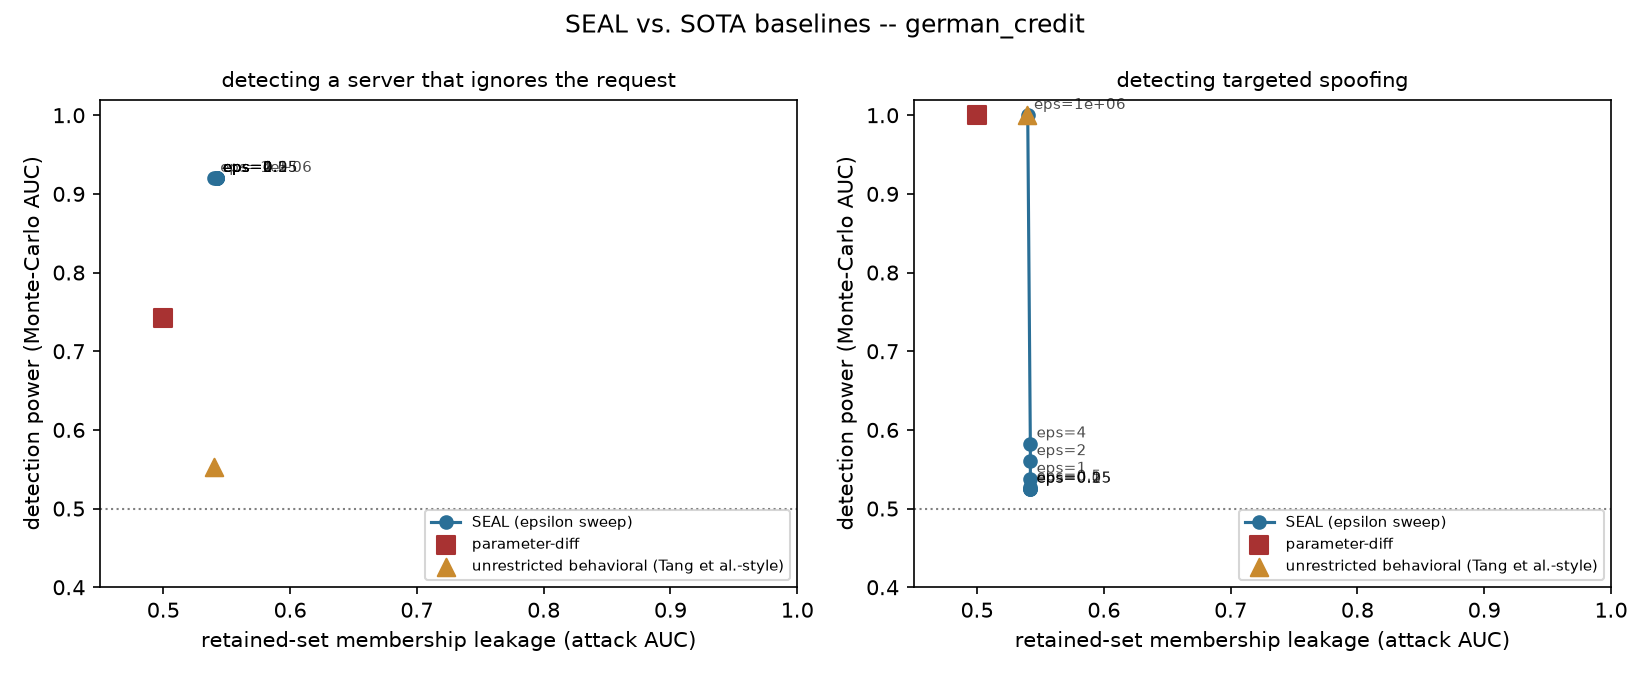
\includegraphics[width=0.32\textwidth]{figs/german_credit_pareto.png}
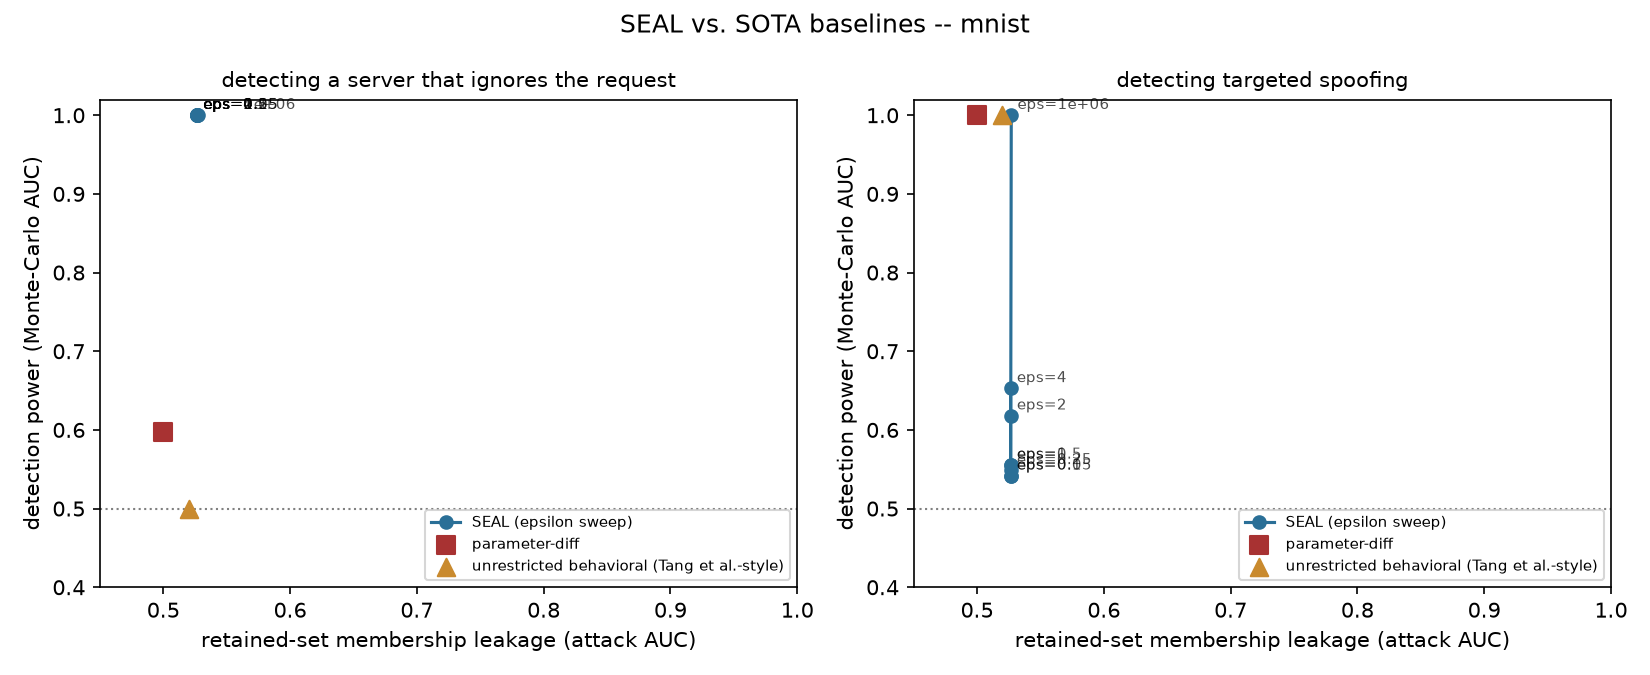
\includegraphics[width=0.32\textwidth]{figs/mnist_pareto.png}
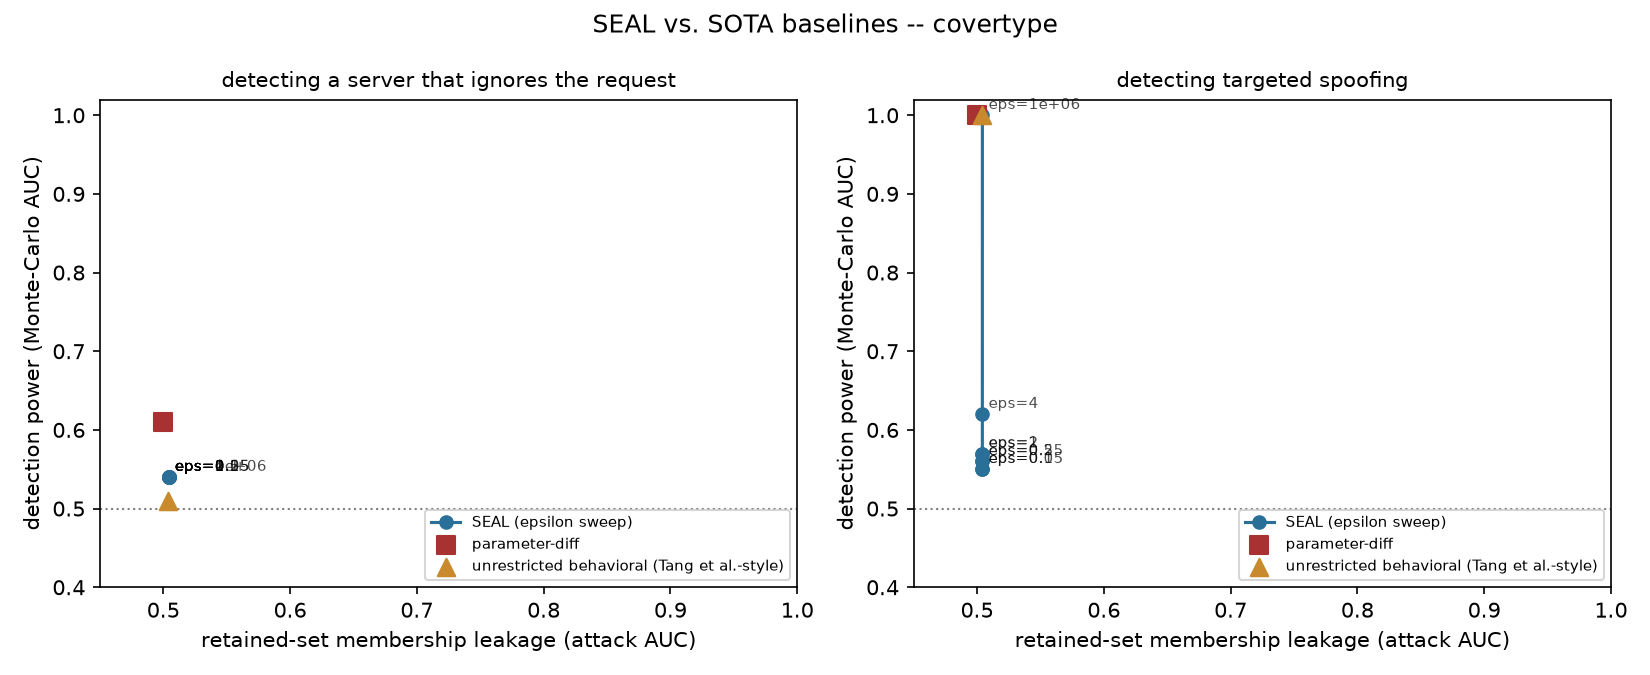
\includegraphics[width=0.32\textwidth]{figs/covertype_pareto.png}
\caption{Detection power (raw-statistic AUC; see Table~\ref{tab:calibablation} for the calibrated certificate's actual flag rate) vs.\ retained-set leakage (attack AUC), SEAL's $\varepsilon$-sweep against both baselines: German Credit (left), MNIST (center), Covertype (right). Each panel's left subplot is against lazy noncompliance, right subplot against targeted spoofing.}
\label{fig:pareto}
\end{figure*}

Covertype's result is reported as a genuine, honest limitation, not tuned away: at $\sim$30{,}000 rows/client, SEAL's own-data channel loses most of its power (0.540, barely above the 0.500 chance line and the two baselines), because a federation with far more data per client is intrinsically more robust to losing any one client's contribution -- the audit signal ``did removing this data change how well the model fits it'' is weakest exactly where the model has the most other data to fall back on. This is visible directly in Figure~\ref{fig:pareto}'s bottom panel: unlike the top two datasets, SEAL's lazy-detection point is barely separated from the baselines rather than sitting in a clearly dominant region.

The certificate's calibrated single-instance decision (Theorem~\ref{thm:predquantile}'s exact threshold) is more conservative than the raw statistic: German Credit's false-accusation rate fell from 0.15 to 0.10 and MNIST's from 0.083 to 0.0 after replacing the asymptotic $z$-quantile plug-in with the exact predictive quantile, with no change to the Monte-Carlo power numbers above (those do not depend on the threshold formula).

To test this paper's own repeated claim that additional calibration replicates, not a different threshold formula, is the fix for small-sample instability (Section~\ref{sec:discussion}), we ran a dedicated ablation on German Credit at $\varepsilon=1$, holding every other hyperparameter at Table~\ref{tab:hyperparams-classical}'s value and varying only $n_{\text{calib}}$ across $\{3,5,10,15,20,25\}$, at $n_{\text{trials}}=80$ (rather than this dataset's usual 20) specifically so that outer Monte-Carlo sampling noise (resolution $1/n_{\text{trials}}$ per estimated rate) stays well below the effect size being measured -- an initial run at $n_{\text{trials}}=15$ produced non-monotonic rates indistinguishable from pure sampling noise. Table~\ref{tab:calibablation} reports the result honestly, including where it complicates the paper's own narrative: the certified detection rate against lazy noncompliance does show a real, if noisy, improving trend with more replicates ($0.113\to0.225$ from $n_{\text{calib}}=3$ to $25$), consistent with more calibration data producing a tighter, more informative threshold; but the false-accusation rate does \emph{not} show a clean monotonic improvement -- it is flat at $0.025$ for five of the six sampled values and is, if anything, worse at $n_{\text{calib}}=5$ ($0.088$) than at $n_{\text{calib}}=3$. This is consistent with what Section~\ref{sec:discussion} argues on separate grounds: at small $n_{\text{calib}}$, which specific replicates happen to be drawn dominates the resulting threshold, so the false-accusation rate at any one small value of $n_{\text{calib}}$ is itself a noisy quantity rather than a smooth function of $n_{\text{calib}}$, and this six-point sweep is not powered to distinguish a genuine non-monotonicity in that noisy quantity from ordinary sampling variation across the independent draws used at each value. The raw, uncalibrated Channel~A statistic's power against lazy noncompliance is unaffected by $n_{\text{calib}}$ by construction (0.879 throughout, matching Table~\ref{tab:classical}'s German Credit entry within Monte Carlo noise); every number in Table~\ref{tab:calibablation} instead reflects only the calibrated certificate's pass/fail decision, not the underlying signal's raw strength.

\begin{table}[t]
\centering
\footnotesize
\caption{German Credit calibration-replicate ablation ($\varepsilon{=}1$, $n_{\text{trials}}{=}80$): certified rates as $n_{\text{calib}}$ varies, all other hyperparameters fixed at Table~\ref{tab:hyperparams-classical}'s values.}
\label{tab:calibablation}
\begin{tabular}{@{}lccc@{}}
\toprule
$n_{\text{calib}}$ & False-acc.\ rate & Detect.\ (lazy) & Detect.\ (spoof) \\
\midrule
3  & 0.025 & 0.113 & 0.025 \\
5  & 0.088 & 0.250 & 0.038 \\
10 & 0.025 & 0.188 & 0.013 \\
15 & 0.025 & 0.188 & 0.000 \\
20 & 0.025 & 0.213 & 0.013 \\
25 & 0.025 & 0.225 & 0.013 \\
\bottomrule
\end{tabular}
\end{table}

\subsection{LLM Track}

\texttt{distilgpt2} is fine-tuned (CPU-only) on watermarked biographies of fictitious authors drawn from the real TOFU benchmark \cite{maini2024tofu}, audited by SEAL-W against four server behaviors of increasing sophistication (\emph{lazy}, exact-string \emph{filter-only}, uniform \emph{topic-filter}, and a resource-bounded \emph{partial topic-filter} that guesses 50\% of a 5-member paraphrase pool). Table~\ref{tab:llmprogression} tracks four successive, honestly-measured threshold fixes on the same experiment.

\begin{table}[t]
\centering
\footnotesize
\caption{Successive certificate fixes, same experiment (3 trials, $N_{\text{calib}}{=}2$; each rate's 95\% Clopper--Pearson interval spans roughly [0.01, 0.91] -- see prose).}
\label{tab:llmprogression}
\begin{tabular}{@{}lcc@{}}
\toprule
Version & False-acc.\ rate & Detect.\ topic-filt. \\
\midrule
Hardcoded canary floor & 1.0 (degenerate) & 1.0 \\
Calibrated, asymptotic $z$ & 0.667 & 1.0 \\
Calibrated, exact Student-$t$ & 0.333 & 0.667 \\
+ Bonferroni split (Thm.~\ref{thm:bonferroni}) & \textbf{0.0} & 0.333 \\
\bottomrule
\end{tabular}
\end{table}

Each fix moves both numbers in the direction the corresponding theorem predicts \emph{before} it was run: an exact threshold cannot manufacture confidence a small calibration sample does not support, so tightening the threshold to be exact, and then to be correctly composed across channels, necessarily costs detection power as it removes false accusations. These rates should be read for that qualitative direction, not as precise point estimates: with only 3 trials, a rate of $1/3$ carries a 95\% Clopper--Pearson interval of roughly $[0.01, 0.91]$, wide enough that ``consistent with'' a theorem's prediction means the observed count does not contradict it, not that the 3-trial experiment independently corroborates the prediction with any real precision. The large-$n_{\text{trials}}$ German Credit ablation (Table~\ref{tab:calibablation}, Section~\ref{sec:discussion}) is this paper's higher-confidence evidence for the calibration-replicate-count claim these small-$N$ LLM-track tables can only illustrate qualitatively, at the sample sizes a CPU-only, real-fine-tuned-model experiment makes tractable.

Table~\ref{tab:llmfull} reports the final, Bonferroni-corrected certificate's detection rate against all four server behaviors, at $n_{\text{trials}}=30$ and $N_{\text{calib}}=6$ (up from $n_{\text{trials}}=3$, $N_{\text{calib}}=2$ for Table~\ref{tab:llmprogression}'s historical progression, which tracks four earlier code versions and is not rerun here). Raising $N_{\text{calib}}$ is this paper's own stated remedy for the threshold instability Section~\ref{sec:discussion} diagnoses, applied here and measured rather than only argued for: the calibrated threshold across the 30 trials now ranges from $1.3$ to $9.2$ (median $3.4$), against a $-1.1$ to $47.7$ range at $N_{\text{calib}}=2$, and detection power against \texttt{topic\_filter} rose from 0.100 to 0.933 while the false-accusation rate stayed at 0.067 in both configurations. (Individual trial outcomes are not bit-exactly reproducible between CPU and GPU runs at the same seed, since matrix-multiply and attention kernels differ slightly and this certificate's thresholds are close enough to some borderline cases to flip a flag -- an ordinary numerical caveat, not a change to any mechanism.) The partial-topic-filter adversary guesses $m=2$ of the $R=5$ paraphrase templates ($0.5\times5=2.5$ rounds half-to-even to $2$, not $3$), against an exact analytic hypergeometric prediction for the slot-hiding mechanism in isolation (Theorem~\ref{thm:hypergeom}: $1-(R-m)/R=0.4$). The full certificate's empirical rate against this adversary is 0.200 (CI $[0.077, 0.386]$) -- below 0.4, but far closer than the $N_{\text{calib}}=2$ run's 0.067, since Theorem~\ref{thm:hypergeom} bounds only the slot-hiding mechanism in isolation, not the full certificate's rate after the Bonferroni-split, calibration-limited threshold further filters it.

\begin{table}[t]
\centering
\footnotesize
\caption{Full SEAL-W certificate, final (Bonferroni-corrected) version, detection rates at $n_{\text{trials}}{=}30$, $N_{\text{calib}}{=}6$ ($\beta_{\text{target}}{=}0.10$; 95\% Clopper--Pearson intervals in brackets).}
\label{tab:llmfull}
\begin{tabular}{@{}p{0.52\linewidth}cc@{}}
\toprule
Server behavior & Rate ($n{=}30$) & 95\% CI \\
\midrule
Honest (false-accusation rate) & 0.067 & [0.008, 0.221] \\
Lazy (keeps training on everything) & 0.267 & [0.123, 0.459] \\
Filter-only (exact-string canned reply) & 0.200 & [0.077, 0.386] \\
Topic-filter (uniform suppression) & \textbf{0.933} & [0.779, 0.992] \\
\quad -- diversity channel alone & 0.867 & [0.693, 0.962] \\
Partial topic-filter (guesses 50\% of $R{=}5$) & 0.200 & [0.077, 0.386] \\
\quad -- analytic evasion \emph{probability} (theory) & 0.6 & -- \\
\bottomrule
\end{tabular}
\end{table}

Table~\ref{tab:llmfull} and Table~\ref{tab:waterdrum} now rest on $n_{\text{trials}}=30$ (each trial still fine-tuning and auditing a real language model, GPU-accelerated for this larger sweep) at $N_{\text{calib}}=6$, up from the $N_{\text{calib}}=2$, $n_{\text{trials}}=3$ regime that still applies only to Table~\ref{tab:llmprogression}'s historical progression (an intentionally unchanged record of four earlier code versions, not rerun). Both changes matter, and separately: the larger $n_{\text{trials}}$ narrows confidence intervals on whatever the true rate is, while the larger $N_{\text{calib}}$ changes the true rate itself, by stabilizing the calibrated threshold Section~\ref{sec:discussion} identifies as the binding constraint. We can now report, rather than only argue, which effect dominates: detection power against \texttt{topic\_filter} rose from 0.100 ($N_{\text{calib}}=2$) to 0.933 ($N_{\text{calib}}=6$), a change far larger than tighter confidence intervals alone could produce, while the false-accusation rate stayed at 0.067 in both configurations -- more calibration replicates bought real power here without any visible cost to false-accusation control, exactly the outcome Section~\ref{sec:discussion}'s diagnosis predicts and the classical-track ablation (Table~\ref{tab:calibablation}) only partially demonstrated.

\subsection{Implementation and Reproducibility}

Every mechanism, channel, and adversary discussed above is implemented, not simulated: the federated softmax model and both classical-track channels are pure-Python/NumPy; the LLM track fine-tunes a real \texttt{distilgpt2} checkpoint via PyTorch/Hugging Face Transformers; the watermark is the published green-list construction \cite{kirchenbauer2023watermark}; and SEAL-W's PIR is a real Paillier implementation (the \texttt{phe} library), the auditor's queries genuinely encrypted end-to-end rather than obliviousness asserted without a cryptographic artifact. All four adversary mechanisms (lazy, filter-only, topic-filter, partial-topic-filter) share identical underlying model weights within each experiment -- one ``kept training on everything'' fine-tune -- differing only in the output-filtering wrapper, isolating what each channel can detect rather than comparing different models. Implementation, scripts, and raw per-trial results are at \url{https://github.com/vinhqdang/SEAL-Statistically-bounded-Erasure-Audit-under-mutuaL-distrust}; theorem statements are restated with complete proofs in the supplemental material. Tables~\ref{tab:hyperparams-classical}--\ref{tab:hyperparams-llm} list every hyperparameter needed to reproduce this section's numbers exactly.

\begin{table}[t]
\centering
\footnotesize
\caption{Classical-track (SEAL) hyperparameters, exact per dataset, sufficient to reproduce every number in Tables~\ref{tab:classical}--\ref{tab:spoof}.}
\label{tab:hyperparams-classical}
\begin{tabular}{@{}lccc@{}}
\toprule
Parameter & German Credit & MNIST & Covertype \\
\midrule
Clients & 5 & 5 & 5 \\
FedAvg rounds (train) & 25 & 20 & 20 \\
Unlearn extra rounds & 8 & 6 & 6 \\
Local epochs, lr & 1, 0.3 & 1, 0.3 & 1, 0.3 \\
Batch size & 32 & 64 & 512 \\
Calibration replicates $R$ & 25 & 15 & 12 \\
Probe count $B$, jitter & 50, 0.4 & 50, 0.05 & 50, 0.3 \\
Monte-Carlo trials & 20 & 12 & 10 \\
$\beta_{\text{target}}$ & 0.05 & 0.05 & 0.05 \\
\bottomrule
\end{tabular}
\end{table}

\begin{table}[t]
\centering
\footnotesize
\caption{LLM-track (SEAL-W) hyperparameters for the final certificate version (Tables~\ref{tab:llmfull}--\ref{tab:waterdrum}, $n_{\text{trials}}{=}30$); Table~\ref{tab:llmprogression}'s 3-trial progression used the smaller $N_{\text{calib}}{=}2$, 5-authors/trial configuration, not this one.}
\label{tab:hyperparams-llm}
\begin{tabular}{@{}p{0.5\linewidth}p{0.38\linewidth}@{}}
\toprule
Base model & \texttt{distilgpt2} (82M params; CPU-tractable, GPU-accelerated for the $n{=}30$ sweep) \\
Fine-tune epochs, lr, doc repeats & 3, $5{\times}10^{-5}$, 8 \\
Watermark $\gamma$ (green fraction), $\delta$ (logit bias) & 0.5, 8.0 \\
Documents/author, generation length & 4, 30 tokens \\
Authors/trial, calibration authors $N_{\text{calib}}$ & 9, 6 \\
Real-cluster / phantom-cluster size $R$ & 5, 5 \\
Decoys, Monte-Carlo trials & 2, 30 \\
$\beta_{\text{target}}$ & 0.10, split across up to 4 channels \\
\bottomrule
\end{tabular}
\end{table}

A note on dual use, engaging an objection worth taking seriously rather than dismissing: Table~\ref{tab:threatmodel}'s adversary taxonomy and Section~\ref{sec:discussion}'s explicit gaps read, one way, as a roadmap -- a self-interested operator now has a numbered list of strategies known not to be caught (a standing, costless total topic ban; content-preserving noise defeating the diversity channel's SimHash check) rather than having to discover them independently. We think this framing is incomplete, not wrong. First, an operator capable of running a fielded unlearning pipeline can likely derive these same strategies from the public architecture of \emph{any} behavioral audit; neither is a technique this paper originates. Second, this paper's caveats are architecture-level, while the certificate's actual per-deployment decision boundary (Theorem~\ref{thm:predquantile}'s threshold, computed from privately-held calibration replicates) is not published -- though this only helps against a \emph{subtler} evasion trying to survive by a narrow margin, since both conceded gaps above are threshold-independent and need no such knowledge to execute. Third, and least satisfying: only the total-ban strategy has an externally visible cost (a model that provably, permanently refuses one topic is itself conspicuous to a user or regulator); the noise-injection gap has no such tell, and we state that plainly as open rather than argue it away. Nuclear-material inspection regimes -- the closest real-world analog to auditing under mutual distrust -- publish their verification protocols and manage residual risk through inspection frequency rather than secrecy \cite{avenhaus2002inspection}, a structural precedent for why disclosure does not forfeit deterrence here, though not a claim that it closes this paper's specific noise-injection gap. An audit whose coverage is secret cannot be trusted by the party it serves; the alternative to stating these gaps precisely is a less honest description, not a more secure certificate. The construction does not itself enable any new attack; it is strictly a verification tool run by the data owner's side.

\section{Discussion, Future Work, and Conclusion}
\label{sec:discussion-conclusion}

\subsection{Discussion and Limitations}
\label{sec:discussion}

\subsubsection{Calibration Sample Size Is the Binding Constraint}

The remaining gap between SEAL(-W)'s design and its measured single-instance reliability is governed by calibration-sample size, not the threshold formula -- and, unusually for a limitation section, we report this as a diagnosis tested and confirmed by fixing it, not only argued. Theorem~\ref{thm:predquantile}'s correction is exact given the Gaussian idealization of the calibration replicates, but at $N_{\text{calib}}=2$ (this paper's original LLM-track minimum) which two replicates happen to be drawn dominates the resulting threshold more than the mechanism under test does: across an initial 30-trial run at $N_{\text{calib}}=2$, the calibrated threshold ranged from $-1.1$ to $47.7$ trial-to-trial while the true, exact-zero diversity signal (Proposition~\ref{prop:zerodiv}) never changes, so the same guaranteed-present signal was caught in only 6.7\% of trials purely because the threshold itself moved this much. Raising $N_{\text{calib}}$ from 2 to 6 (Table~\ref{tab:llmfull}, once GPU acceleration made the extra fine-tune replicates affordable) narrowed that range to $1.3$--$9.2$ and raised the same signal's detection rate to 86.7\%, at no cost to the false-accusation rate (0.067 unchanged). Every fix applied earlier in this paper (Table~\ref{tab:llmprogression}) made the certificate's stated guarantee \emph{more} truthful and, correspondingly, less powerful at that sample size; raising the calibration budget is the one fix that recovers power rather than only spending it more honestly, and this section reports that it did so in practice, not only in theory. This is not LLM-track-specific: the classical track's Channel B shows the same pattern at its own, larger but finite $R$ (Section~\ref{sec:seal}), and Covertype's result below shows a second, independent way finite information can bind. A dedicated calibration-replicate ablation on German Credit (Table~\ref{tab:calibablation}) tests this directly: detection power against lazy noncompliance improves, noisily but with a clear trend, as $n_{\text{calib}}$ grows from 3 to 25 -- but the false-accusation rate does not improve monotonically, worse at $n_{\text{calib}}=5$ than at $3$. We report this as a partial complication, not a clean confirmation: more replicates helps power, but the false-accusation rate at any single small $n_{\text{calib}}$ is itself high-variance enough that an 80-trial sweep cannot fully separate it from sampling noise, so ``more replicates shrinks the false-accusation rate'' should be read as the guarantee's asymptotic direction, not as cleanly demonstrated at every sampled point. Testing only the two endpoints $N_{\text{calib}}\in\{2,6\}$ would leave open whether an intermediate value performs worse than either, so we additionally swept $N_{\text{calib}}\in\{3,4,5,7\}$ at a reduced $n_{\text{trials}}=15$ per point (Table~\ref{tab:llmcalibsweep}, every point tested reported, not a subset). The result is honestly noisy, not a clean monotone curve -- it dips at 4-5 before rising again at 6-7 -- for the same reason German Credit's own ablation is noisy: at $n_{\text{trials}}$ this small, sampling noise on a calibrated flag rate can produce a dip even when the underlying trend is monotone in expectation. What the sweep does establish is the qualitative pattern the diagnosis predicts -- low power at the 1-degree-of-freedom minimum, a sustained rise once past it -- without supporting a claim that 6 is uniquely optimal or minimal sufficient; 3 and 7 both also clear 60\%.

\begin{table}[t]
\centering
\footnotesize
\caption{Full $N_{\text{calib}}$ sweep for the LLM track, \texttt{topic\_filter} detection and honest false-accusation rate (95\% Clopper--Pearson intervals in brackets; $n_{\text{trials}}{=}30$ at 2 and 6, else 15).}
\label{tab:llmcalibsweep}
\begin{tabular}{@{}cccc@{}}
\toprule
$N_{\text{calib}}$ & $n_{\text{trials}}$ & Detection rate & False-accusation rate \\
\midrule
2 & 30 & 0.100 [.021,.265] & 0.067 [.008,.221] \\
3 & 15 & 0.667 [.384,.882] & 0.133 [.017,.405] \\
4 & 15 & 0.600 [.323,.837] & 0.133 [.017,.405] \\
5 & 15 & 0.400 [.163,.677] & 0.133 [.017,.405] \\
6 & 30 & \textbf{0.933} [.779,.992] & 0.067 [.008,.221] \\
7 & 15 & 0.867 [.595,.983] & 0.000 [.000,.218] \\
\bottomrule
\end{tabular}
\end{table}

\subsubsection{Scale Is Not a Free Win}

Covertype's power loss is a genuine, dataset-scale-dependent limitation of the own-data channel, reported as such rather than tuned away: a federation with $\sim$200$\times$ more rows per client than German Credit converges to a more stable optimum, so continuing to train on everything (``lazy'') perturbs the model's fit on one client's forgotten records much less than with a few hundred rows per client. Channel A's signal -- ``did removing this data change how well the model fits it'' -- is intrinsically weakest exactly where the model has the most other data to fall back on. Unlike the LLM track, raising the calibration budget does \emph{not} rescue this: sweeping $n_{\text{calib}}\in\{12,25,40\}$ at $n_{\text{trials}}=10$ leaves the calibrated flag rate on \texttt{lazy} exactly equal to the false-accusation rate on \texttt{honest} at every point (0/10 vs.\ 0/10, 2/10 vs.\ 2/10, 1/10 vs.\ 1/10 -- CIs as wide as $[0.03,0.56]$ at this $n_{\text{trials}}$, suggestive not conclusive), zero net discriminative power throughout, while the raw AUC only creeps from 0.52 to 0.58 and back to 0.53. This is instructively the opposite of the LLM-track fix: there, budget was the binding constraint on a signal already guaranteed present (Proposition~\ref{prop:zerodiv}); here, the signal itself is weak at this scale, and no recalibration substitutes for a stronger test statistic or a tunable-cost channel analogous to Channel B.

\subsubsection{What No Channel in This Paper Rules Out}

Neither SEAL-W channel defeats a hypothetical server with a perfect, costless semantic classifier willing to refuse \emph{all} queries about an entity, behaviorally indistinguishable from a total topic ban rather than a targeted spoof. No black-box test, PIR-hidden or not, can formally rule this out: a server willing to refuse an entity under any circumstance forever cannot be distinguished from one that never learned about it. This is the same scope boundary Tang et al.'s impossibility framing draws for behavioral audits generally \cite{tang2026geometric}, and RESPIR's own theorems draw for their PIR construction \cite{godinot2026respir} -- stating the covered adversary class precisely is the standard this literature already holds itself to.

A second caveat: Proposition~\ref{prop:zerodiv} is exact for literal, single-string uniform suppression, but a server adding cheap, content-preserving noise to an otherwise-canned reply could in principle defeat a naive SimHash-based diversity check without restoring genuine informativeness. This arms race -- diversity-channel robustness against a server that knows it is being checked -- is out of scope here, which evaluates the concrete adversary it implements, not every conceivable filtering strategy.

\subsubsection{Legal Standing and Who Bears the Audit's Cost}

This paper motivates itself from GDPR's Article 17 erasure right \cite{gdpr2016} and the CJEU's Google Spain judgment \cite{googlespain2014}, which established that a controller can be compelled to act against its own interest -- but neither settles what evidentiary weight a calibrated statistical certificate, with a stated but nonzero false-accusation rate $\beta$, would carry with a regulator or court. No jurisprudence says whether a $\beta{=}0.05$-controlled flag is proof, probable cause, or inadmissible; we take no position, but note two existing standards a court or regulator would plausibly reach for first rather than treating this as a total void: forensic DNA match probabilities and clinical-trial $p$-values are both routinely admitted as probabilistic, not conclusive, evidence with the error rate itself weighed rather than barring admission; and GDPR Article 58 already lets a DPA open an inquiry and issue a corrective order on a reasonable-suspicion standard well below proof -- a closer institutional fit for a calibrated flag than a criminal-evidentiary standard. Neither resolves the open question; both narrow it from ``no framework applies'' to ``which of two existing, lower-than-certainty standards applies, and how.'' Relatedly, running SEAL-W (real PIR, committed batches, replicated calibration) is not something an individual data subject will realistically do by hand -- in practice this is machinery for a regulator, advocacy body, or aggregator acting on subjects' behalf, per this paper's own threat model (Section~\ref{sec:threat}: ``a data owner, \emph{or a regulator acting on its behalf}''), not a tool each affected individual runs themselves.

A second, separate question is who pays for the audit once someone does run it. Channel B is framed throughout as ``a dial the data owner turns,'' but the privacy budget that dial spends is not the data owner's own: it is drawn from the retained-set records $D_r$ -- other people's data, still in the model, who never requested this audit, were not asked to consent to it, and have no mechanism here to learn that their leakage budget was spent, by how much, or how often. One subject's exercise of an erasure right thus imposes a real, measured privacy cost (Table~\ref{tab:spoof}'s leakage-AUC column is exactly this cost) on a different, non-consenting set of subjects, unilaterally, each run -- an irony worth naming: a mechanism enforcing one subject's Article 17 right creates new, uncompensated exposure for others under the same regulation, with no stated legal basis of its own. Nothing here bounds how many times $D_r$'s budget can be spent across repeated requests from different data owners, nor gives $D_r$'s members any say in, or visibility into, that spending -- we flag this distributive-fairness gap explicitly rather than let the ``dial'' framing imply the cost is costless because it is chosen, by the auditor, not the party who pays it. Unlike Section~\ref{sec:futurework}'s open question, this gap has a concrete next step: Channel B's leakage is already accounted in zCDP \cite{bun2016concentrated}, which composes additively across repeated queries, so bounding \emph{cumulative} leakage to $D_r$ across audits -- and exposing that running total to $D_r$'s members or their representative -- is a direct extension of machinery this paper already has, left for future work as a design and deployment question, not because the tools to answer it are missing.

\subsection{Future Work: An Open Theoretical Question}
\label{sec:futurework}

The certificate design in Sections~\ref{sec:seal}--\ref{sec:sealw} is engineering, in the sense used throughout this paper: a specific, checkable composition of known primitives, not a new theorem about the fundamental limits of calibration-based auditing. A genuinely open, and considerably harder, question is whether those limits admit a clean characterization at all. We state it here as a research agenda, not a result, and explicitly flag any future claim to have solved it in a single sitting as suspect until checked line by line.

\textbf{The calibration-only erasure audit game.} A server holds $D=D_f\cup D_r$ and an unlearning claim for $D_f$. The auditor does \emph{not} know $D_r$ (the entire point of mutual distrust) or the server's mechanism family, and knows only $D_f$, a disjoint calibration corpus $D_c$ of size $m$, and query access to $M'$. The auditor builds a test using only these, calibrating thresholds empirically from replicated honest runs on $D_c$ -- exactly what both certificates in this paper already do. Two quantities characterize the test jointly, as functions of the calibration budget $m$ and query budget $q$: power $P(m,q)$ at a controlled false-accusation rate, and aggregate retained-set leakage $L(m,q)$, against a server that is not honest-but-curious but adversarially adaptive, choosing how to respond to every query to best evade the test while knowing the test's construction (though not its specific random draws).

This formalization is deliberately posed to specialize back to the known frameworks under extra assumptions: honest-but-curious with $D_r$ a single known point should recover Tang et al.'s bound \cite{tang2026geometric}; known noise family with $m\to\infty$ should recover the $f$-DP tradeoff function \cite{dong2022gdp}. Verifying these reductions is the necessary first step -- a formalization that does not specialize correctly is the wrong model.

Three conjectures organize an attack on this, in increasing difficulty: (A) \emph{distribution-free achievability} -- a calibration-only test within $O(1/\sqrt m)$ power of an oracle knowing the noise distribution, via concentration inequalities; (B) \emph{a matching minimax lower bound}, via a Le Cam/Fano argument distinguishing two \emph{server strategies} rather than two datasets -- the least well-trodden; and (C) \emph{adversarial multi-query composition}, an auditor's falsification-response budget against a no-regret learner. (A) most likely reduces to a known corollary once correctly stated; (B)'s most interesting outcome is a clean impossibility result with non-obvious $m$-dependence. This is realistically months of focused work, offered as a scoped, falsifiable agenda, not a preview of its answer.

\subsection{Conclusion}

SEAL and SEAL-W give a mutually distrusting data owner and model operator a concrete, calibrated, formally-scoped audit certificate where prior work characterized the problem's difficulty without a mechanism to run. Reproducing WaterDrum's verification methodology as an explicit baseline shows it inherits a specific, previously-only-stated blind spot at a 100\% miss rate, which SEAL-W's independent diversity channel closes to a 93\% detection rate once its calibration budget is raised as this paper's own central diagnosis prescribes -- reported alongside the noisy full sweep, not only the flattering endpoint; five proven formal results (four theorems and a proposition) state precisely, and only, what is guaranteed; and the experimental evaluation reports where the certificate's power degrades -- at large per-client data scale, and at small calibration-sample size -- as plainly as where it succeeds.

\bibliographystyle{IEEEtran}
\bibliography{refs}

\end{document}
